\documentclass[a4paper,
fontsize=11pt,
%headings=small,
oneside,
numbers=noperiodatend,
parskip=half-,
bibliography=totoc,
final
]{scrartcl}

\usepackage{synttree}
\usepackage{graphicx}
\setkeys{Gin}{width=.4\textwidth} %default pics size

\graphicspath{{./plots/}}
\usepackage[ngerman]{babel}
\usepackage[T1]{fontenc}
%\usepackage{amsmath}
\usepackage[utf8x]{inputenc}
\usepackage [hyphens]{url}
\usepackage{booktabs} 
\usepackage[left=2.4cm,right=2.4cm,top=2.3cm,bottom=2cm,includeheadfoot]{geometry}
\usepackage{eurosym}
\usepackage{multirow}
\usepackage[ngerman]{varioref}
\setcapindent{1em}
\renewcommand{\labelitemi}{--}
\usepackage{paralist}
\usepackage{pdfpages}
\usepackage{lscape}
\usepackage{float}
\usepackage{acronym}
\usepackage{eurosym}
\usepackage[babel]{csquotes}
\usepackage{longtable,lscape}
\usepackage{mathpazo}
\usepackage[normalem]{ulem} %emphasize weiterhin kursiv
\usepackage[flushmargin,ragged]{footmisc} % left align footnote
\usepackage{ccicons} 
\setcapindent{0pt} % no indentation in captions

%%%% fancy LIBREAS URL color 
\usepackage{xcolor}
\definecolor{libreas}{RGB}{112,0,0}

\usepackage{listings}

\urlstyle{same}  % don't use monospace font for urls

\usepackage[fleqn]{amsmath}

%adjust fontsize for part

\usepackage{sectsty}
\partfont{\large}

%Das BibTeX-Zeichen mit \BibTeX setzen:
\def\symbol#1{\char #1\relax}
\def\bsl{{\tt\symbol{'134}}}
\def\BibTeX{{\rm B\kern-.05em{\sc i\kern-.025em b}\kern-.08em
    T\kern-.1667em\lower.7ex\hbox{E}\kern-.125emX}}

\usepackage{fancyhdr}
\fancyhf{}
\pagestyle{fancyplain}
\fancyhead[R]{\thepage}

% make sure bookmarks are created eventough sections are not numbered!
% uncommend if sections are numbered (bookmarks created by default)
\makeatletter
\renewcommand\@seccntformat[1]{}
\makeatother

% typo setup
\clubpenalty = 10000
\widowpenalty = 10000
\displaywidowpenalty = 10000

\usepackage{hyperxmp}
\usepackage[colorlinks, linkcolor=black,citecolor=black, urlcolor=libreas,
breaklinks= true,bookmarks=true,bookmarksopen=true]{hyperref}
\usepackage{breakurl}

%meta

%meta

\fancyhead[L]{Redaktion LIBREAS \\ %author
LIBREAS. Library Ideas, 35 (2019). % journal, issue, volume.
\href{http://nbn-resolving.de/}
{}} % urn 
% recommended use
%\href{http://nbn-resolving.de/}{\color{black}{urn:nbn:de...}}
\fancyhead[R]{\thepage} %page number
\fancyfoot[L] {\ccLogo \ccAttribution\ \href{https://creativecommons.org/licenses/by/4.0/}{\color{black}Creative Commons BY 4.0}}  %licence
\fancyfoot[R] {ISSN: 1860-7950}

\title{\LARGE{Erinnerung an Uwe Müller}} % title
\author{Redaktion LIBREAS} % author

\setcounter{page}{1}

\hypersetup{%
      pdftitle={Erinnerung an Uwe Müller},
      pdfauthor={Redaktion LIBREAS},
      pdfcopyright={CC BY 4.0 International},
      pdfsubject={LIBREAS. Library Ideas, 35 (2019).},
      pdfkeywords={Nachruf, Uwe Müller, obituary},
      pdflicenseurl={https://creativecommons.org/licenses/by/4.0/},
      pdfcontacturl={http://libreas.eu},
      baseurl={http://libreas.eu},
      pdflang={de},
      pdfmetalang={de}
     }



\date{}
\begin{document}

\maketitle
\thispagestyle{fancyplain} 

%abstracts

%body
\hypertarget{gemeinsam-erinnern}{%
\section{Gemeinsam Erinnern}\label{gemeinsam-erinnern}}

Am 22. Februar 2019 ist unser Kollege, Chef, Dozent und Freund Uwe
Müller überraschend und unerwartet verstorben. Die LIBREAS-Redaktion
möchte Uwe an dieser Stelle eine Erinnerungsseite widmen und bedankt
sich sehr bei allen, die sich beteiligt haben. Wir wissen, welch
schwierige Aufgabe das Erinnern an einen Menschen ist, der so plötzlich
nicht mehr bei uns ist. Einige versuchen ihre Trauer mithilfe von Worten
zu verarbeiten, andere eher im Stillen. Die Kolleginnen und Kollegen an
Uwes letzter Wirkungsstätte haben in ihren Nachrufen bereits seinen
Einfluss auf die Deutsche Nationalbibliothek (DNB) beziehungsweise die
Deutsche Digitale Bibliothek gewürdigt:

\begin{itemize}
\item
  \enquote{Dr.~Uwe Müller (1975--2019) -- In Memoriam}
  \url{https://www.dnb.de/DE/Aktuell/Personelles/Nachrufe/nachrufUweMueller.html}
\item
  \enquote{Die DDB trauert um Uwe Müller}
  \url{https://www.deutsche-digitale-bibliothek.de/content/journal/aktuell/die-ddb-trauert-um-uwe-mueller/}
\item
  \enquote{Zum Gedenken an Uwe Müller (1975 bis 2019)} In: Dialog mit
  Bibliotheken, 31(1) 2019, S. 78--79.
  \url{https://nbn-resolving.org/urn:nbn:de:101-2019022814}
\end{itemize}

Vor seiner Tätigkeit an der DNB war Uwe Müller im Computer- und
Medienservice und dem Institut für Bibliotheks- und
Informationswissenschaft der Humboldt-Universität zu Berlin beschäftigt.
Außerdem war er seit vielen Jahren eine zentrale Person in der DINI-AG
Elektronisches Publizieren -- sowohl für die inhaltliche Ausgestaltung
als auch für die hier aktiven Kolleginnen und Kollegen. Er hat uns mit
Ideen angesteckt, und dann kontinuierlich dafür gesorgt, dass aus Ideen
auch Wirklichkeit wird.

Uwe hat auch die LIBREAS-Redaktion von Beginn seiner Tätigkeit am IBI
2006 an sehr unterstützt -- in praktischen Fragen, aber auch in ideeller
Hinsicht. Danke lieber Uwe!

Dieser Beitrag startete mit Erinnerungen von Menschen aus der
LIBREAS-Redaktion, des IBI und der DINI-AG Elektronisches Publizieren
und wurde ergänzt durch weitere Kolleginnen und Kollegen, die sich gerne
noch einmal persönlich an Uwe erinnern wollen. Der Beitrag wurde offen gehalten bis zum Redaktionsschluss der nächsten Ausgabe, um weiteren Personen die Möglichkeit zu geben eine Erinnerung beizusteuern.

\hypertarget{persuxf6nlich-erinnern}{%
\section{Persönlich Erinnern}\label{persuxf6nlich-erinnern}}

\textbf{Peter Schirmbacher: Dr.~Uwe Müller -- eine Würdigung}

Großes Entsetzen und tiefe Betroffenheit waren auch bei mir die
Reaktionen, als ich vom Tod von Uwe Müller erfahren habe. Ich will es
nicht wahrhaben, dass Uwe nicht mehr unter uns weilt. Ich habe ihn als
einen höchst sympathischen, offenen und kollegialen Menschen erlebt, der
sich durch ein hohes Verantwortungsgefühl sowohl für die anstehenden
Aufgaben als auch durch ein großes Einfühlungsvermögen für die ihn
umgebenden Menschen auszeichnete.

Ich kenne Uwe Müller seit 1994, denn er war gemeinsam mit meinem Sohn in
einer Abiturklasse am Heinrich-Hertz-Gymnasium in Berlin. Wenige Jahre
später hatte ich dann die Bewerbungsunterlagen als studentische
Hilfskraft des Informatik-Studenten Uwe Müller auf meinem Tisch. Gesucht
hatte ich eine Hilfskraft mit gehobenen Programmierkenntnissen zur
Mitarbeit in einem der ersten Projekte zum elektronischen Publizieren,
das die Deutsche Forschungsgemeinschaft an den Computer- und
Medienservice (CMS) der Humboldt-Universität vergeben hatte. Im Rahmen
von \enquote{Dissertationen Online} war an der Humboldt-Universität ein
Repositorium für digital vorliegende Dissertationen aufzubauen, das
heißt das technische Gerüst zu gestalten. Uwe Müller hat diese Stelle
bekommen und die Aufgaben mit Bravour erfüllt. Mir war bewusst, dass ich
einen jungen Mann eingestellt hatte, der ein exzellentes fachliches
Wissen auf dem Gebiet der Informatik vorweisen konnte, der in jeder
Phase des Projektes konstruktiv und mit großem Ideenreichtum am Werk war
und dem man zu 100 Prozent vertrauen konnte. Mehr noch als diese
fachlichen Eigenschaften ist jedoch hervorzuheben, dass er von Beginn
seiner Tätigkeit an versucht hat, sich in die Situation der Nutzer der
Ergebnisse seiner Programmierung zu versetzen und deren Anforderungen
kreativ umzusetzen. Ende der 90 er Jahre war das Verständnis der
Informatiker im Umgang mit den Anforderungen aus der Bibliotheks- und
Informationswissenschaft nur wenig entwickelt. So war Uwe an vielen
Stellen Vorreiter.

Aus der studentischen Hilfskraft wurde wenig später der
wissenschaftliche Mitarbeiter im DFG-geförderten Projekt. Die
Entscheidung, die Projektstelle mit Uwe Müller zu besetzen, fiel mir
nicht schwer. Er hat sich innerhalb der Arbeitsgruppe
\enquote{Elektronisches Publizieren}, einer gemeinsamen Arbeitsgruppe
des Computer- und Medienservice und der Universitätsbibliothek, eine
Position erarbeitet, die ihn nahezu unersetzbar machte. Als Beispiel
seiner besonderen Fähigkeiten und seiner Einsatzbereitschaft sei das
Projekt \enquote{XML-Portal für multimediale Objekte} genannt. Dieses
Projekt diente dem exemplarischen Aufbau eines Internet-Portals zur
Erschließung, Archivierung und Recherche von komplexen Dokumenten mit
multimedialen Inhalten unter Nutzung XML-basierter Technologien am
Beispiel des Publikationsservers und der Sammlungsobjekte der
Humboldt-Universität. Uwe Müller hat den DFG-Antrag seinerzeit
federführend geschrieben und ich habe es davor und auch danach nicht
noch einmal erlebt, dass ein Antrag ohne jede Rückfrage, Kürzung oder
Änderung durch die Gutachter der DFG seine Befürwortung gefunden hat. Es
war sein zielstrebiger und gewissenhafter Arbeitsstil, der ihn zu einem
besonderen Mitarbeiter machte.

Als ich 2006 die Gelegenheit bekam, am Institut für Bibliotheks- und
Informationswissenschaft der Humboldt-Universität einen Lehrstuhl für
Informationsmanagement aufzubauen, habe ich mich sehr gefreut, dass Uwe
Müller mein Angebot, als wissenschaftlicher Mitarbeiter im Lehrstuhl zu
arbeiten, annahm. Es war sehr viel Arbeit neben der Tätigkeit im CMS und
in der Arbeitsgruppe \enquote{Elektronisches Publizieren} dem Lehrstuhl
ein Forschungsprofil zu geben und die entsprechenden Vorlesungen und
Seminare zu entwickeln. Uwe war eine höchst verlässliche Stütze mit
einer Vielzahl von Ideen und mit einem besonderen Geschick in der Lehre
auch die Studierenden für unser Fachgebiet zu begeistern.

Uwe Müller hatte den Blick für nationale und internationale
Entwicklungen auf dem Gebiet der Bibliotheksinformatik, sodass es für
die Community ein großes Glück war, dass Uwe gemeinsam mit Frank Scholze
die Leitung der DINI-AG Elektronisches Publizieren nach meinem
Ausscheiden übernahm. Wir alle sind ihm für seinen Einsatz und seine
umsichtige Führung zu großem Dank verpflichtet.

\begin{figure}
\centering
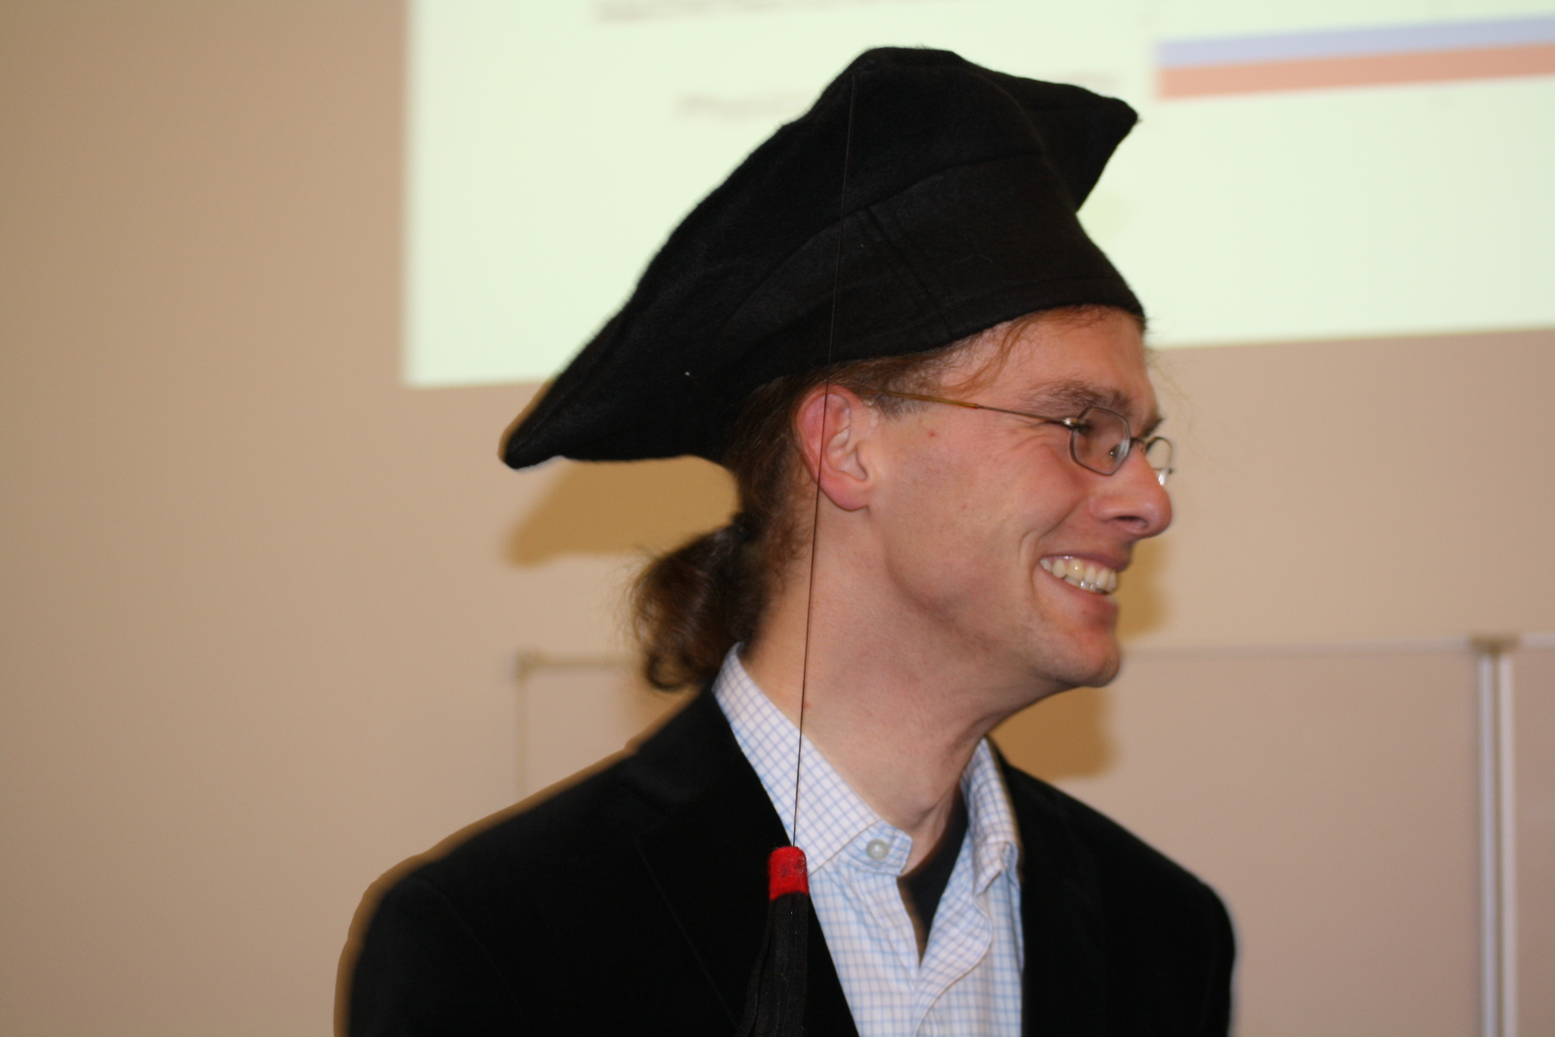
\includegraphics{abb.jpg}
\caption{Uwe Müller}
\end{figure}

Mit seiner Fähigkeit, sich selbst zu organisieren und zu disziplinieren,
hat er in extrem kurzer Zeit eine sehr gute Dissertation verfasst. Mit
dieser Qualifikation und seinem exzellenten Ruf als Informatiker mit
herausragenden bibliothekswissenschaftlichen Kenntnissen standen ihm in
Berlin alle Türen offen. Er hat sich, seinem Wesen entsprechend, für die
Familienzusammenführung entschieden und ist in den Frankfurter Raum
gewechselt. So bedauerlich sein Weggang war, so sehr habe ich mich für
ihn gefreut, dass er mit der Stelle letztlich als Technischer
Geschäftsführer bei der Deutschen Digitalen Bibliothek eine ihm adäquate
Position besetzen konnte.

Uwe Müller wird mir immer als ein liebenswerter, umsichtiger und hoch
kompetenter Mensch in Erinnerung bleiben.

\begin{center}\rule{0.5\linewidth}{0.5pt}\end{center}

\textbf{Ellen Euler}

Ich hatte das Privileg Uwe nicht nur beruflich kennenzulernen (an seiner
Seite habe ich die Geschäftsstelle der Deutschen Digitalen Bibliothek in
Berlin auf- und mit zur Geschäftsführung ausgebaut, während er den
Frankfurter Standort vorangebracht und später als Geschäftsführer
vertreten hat), sondern auch ein klein bisschen privat, als liebenden
Ehemann und Vater.

Er hat in sich \enquote{eine einzigartige Kombination aus positiven
Attributen vereint und mit seiner Kompetenz die DDB und seiner
Menschlichkeit sein Umfeld geprägt}. Uwe Müller habe ich erlebt als:
\textbf{U}neitel, \textbf{W}issend, \textbf{E}mpathisch,
\textbf{M}itdenkend, \textbf{Ü}berdurchschnittlich engagiert,
\textbf{L}ösungsorientiert, \textbf{L}iebenswert, \textbf{E}iner für
alle, \textbf{R}uhig.

Man konnte ihm bedingungslos vertrauen. Er hat niemals (!) negativ über
andere gesprochen und höchstens sein Unverständnis über manche
Herangehensweise geäußert. In allen Angelegenheiten, die wir gemeinsam
zu bearbeiten hatten, war er immer lösungsorientiert, sehr geduldig und
ausdauernd und hat zwischen allen beteiligten Interessen vermittelnd,
dabei nie die Sache aus dem Blick verlierend, gehandelt. Dabei war er
immer aufmerksam genug, um auch die weniger starken Interessen nie zu
übergehen. Kollegen wie Uwe Müller ermöglichen Teams, selbst in einem
stressigen Arbeitsumfeld Höchstleistungen zu bringen und machen aus
auswegslosen Situationen bewältigbare Aufgaben. Egal was anstand, konnte
man sich jederzeit an ihn wenden und viele haben das getan. Ob Kollegen
oder Freunde, er hatte für alle Projektideen, Probleme oder schwierige
Lagen den passenden und weiterführenden Hinweis. Er hat sich dabei nie
wichtig genommen, war es aber immer.

Uwe hat nie etwas lautstark eingefordert, sondern immer auf Einsicht,
Verständnis und Unterstützung gehofft. Er war überzeugt, in einem Markt
an Meinungen würden sich die besten durchsetzen. Manchmal hat das
länger, manchmal weniger lange gedauert, manchmal hat es nicht geklappt.
Vieles musste er selbst regeln und lösen. Da kam dann oft vieles
zusammen.

Wir haben manches Mal darüber sinniert, wie es gelingen kann, für die
eigenen Freunde, die eigenen Kinder, den geliebten Ehepartner oder
pflegebedürftige engste Angehörige da zu sein und gleichzeitig beruflich
24/7 so zu wirken, als gäbe es das alles nicht. Gesprochen haben wir
auch über den gesellschaftlichen und politischen Rahmen, in dem sich
Familie, Beruf und Sozialleben abspielen und in dem sich
Geschlechterrollen auflösen, der Klimawandel Zukunftspläne in Frage
stellt und Familienzusammenführungen aufgrund explodierender Preise für
Mieten zur Unmöglichkeit werden. Wie hierauf reagieren? Anspruchsvoll,
visionär und sozial? Der Spagat zwischen Familie, Beruf und sozialem,
gesellschaftspolitischem (bei ihm zusätzlich kirchlichen) Engagement
zerreißt einen heute. Ob als Mutter oder Vater.

Wir haben keine zufriedenstellende Antwort gefunden. Vielleicht würde es
helfen, wenn wir alle im Rahmen unserer Möglichkeiten seine Werte
weiterleben und uns gegenseitig nicht nur unterstützen, sondern alle
nicht so wichtig nehmen. Was richtig ist, bleibt es auch dann, wenn es
von anderen nicht er- oder anerkannt wird! Das wusste Uwe. Und wir
müssen es uns täglich bewusst machen.

Dabei sollten wir aufmerksam sein, auch für die Familien, die Berufe und
damit einhergehende Verantwortung mit tragen müssen.
Familienvereinbarkeit darf nicht nur eine Floskel sein.

Uwe, hab vielen Dank! Auch Deiner Familie, die alles, was Du
vorangetrieben hast, mit möglich gemacht hat, vielen Dank und mein
tiefstes Mitgefühl!

\begin{center}\rule{0.5\linewidth}{0.5pt}\end{center}

\textbf{Heinz Pampel}

Im Februar 2008 sendete ich meine erste E-Mail an Uwe Müller. Damals war
ich gerade mal seit drei Monaten bei Helmholtz für das Thema Open Access
zuständig. Die damalige E-Mail nahm Bezug auf einen Vortrag von Uwe
Müller über das Meldesystem für Texte auf Internetseiten (METIS) der VG
Wort und den damit verbundenen Herausforderungen für
Open-Access-Repositorien. Es war einer der sehr kompetenten Vorträge von
Uwe Müller, vom denen ich in den folgenden Jahren auf Sitzungen,
Workshops und Konferenzen viele miterleben durfte.

Im selben Jahr begann meine Mitarbeit in der DINI-Arbeitsgruppe
Elektronisches Publizieren. In diesem Kontext erlebte ich Uwe Müller als
immer fachkundigen und sehr beliebten Kollegen, der seine Sprecherrolle
der DINI-AG Elektronisches Publizieren in beeindruckender Weise
ausfüllte. Seine besonnene und vermittelnde Art war in vielen Sitzungen
ein großer Gewinn.

Ganz besonders erinnere ich mich an ein Gespräch mit Uwe Müller in
Adlershof. Auf dem Flur des Computer- und Medienservice der
Humboldt-Universität zu Berlin erzählte ich ihm von meiner ersten groben
Idee eines \enquote{Registry of Research Data Repositories}. Ich, damals
noch wenig erfahren im Drittmittelgeschäft, stieß auf sein offenes Ohr.
Er reagierte damals sehr aufgeschlossen und ermutigend und leistete in
Folge einen wichtigen Beitrag zur Realisierung der Idee.

Eine ähnliche Situation ergab sich einige Jahre später, als mit weiteren
Kollegen die ersten Ideen zu einem gemeinsamen Projekt rund um das Thema
Autorenidentifikation reiften und Uwe Müller die für das Vorhaben
wichtigen Kontakte in die Deutsche Nationalbibliothek vermittelte.

Unsere Zusammenarbeit in diesen beiden Projekten und in vielen anderen
Kontexten, zum Beispiel rund um das DINI-Zertifikat oder auch in der
Kommission Zukunft der Informationsinfrastruktur (KII), war immer
vertrauensvoll, verlässlich und verbindlich.

Der Tod von Uwe Müller hat mich sehr getroffen. Sein Tod ist ein
unfassbarer Verlust.

\begin{center}\rule{0.5\linewidth}{0.5pt}\end{center}

\textbf{Maxi}

Wenn ich an Uwe denke, dann denke ich an ein Verstehen ohne viele Worte.
Was Uwe sagte, hatte Hand und Fuß. Es kam nur selten vor, dass er viel
mehr erzählte, als es die Situation erforderte. Er hat sich selbst oft
sehr zurückgenommen. Seinen Gesprächspartner*innen ist er immer auf
Augenhöhe begegnet, respektvoll, vielleicht manchmal schmunzelnd
kommentierend. Uwe hatte die Gabe, Kollegen niemals das Gefühl zu geben,
auf dem falschen Weg zu sein, sondern hat sie in einer Weise
unterstützt, an der sie wachsen konnten. Dafür bin ich Uwe sehr dankbar.

Diese Zusammenarbeit mit Uwe ist für mich rückblickend von einer Ebene
der Verständigung und Wertschätzung und dem Teilen der Begeisterung für
Themen und Standpunkte geprägt, die eben ohne viele Worte auskam. Eine
Ebene, in der wir gegenseitig eine Lebenshaltung anerkannt haben, sich
wenn dann mit möglichst vollem Einsatz einzubringen.

Ich würde mir jetzt wünschen, dass ich Uwe doch noch manches Wort
darüber hinaus sagen könnte.

Die Lücke, die Uwe hinterlässt, lässt sich nicht wieder füllen. Aber
seine Leidenschaft und Hingabe für Themen wie die Offenheit und
Nachsichtigkeit im Umgang miteinander und die Offenheit in Wissenschaft
und Kultur können wir auch in seinem Namen weiterführen.

\begin{center}\rule{0.5\linewidth}{0.5pt}\end{center}

\textbf{Michaela Voigt}

Vermutlich im Wintersemester 2008/09 habe ich zuerst in deinen
Vorlesungen beziehungsweise Seminaren gesessen, in einem
Wahlpflichtmodul des ersten Bachelor-Jahrgangs mit dem vielsagenden (?)
Titel \enquote{Angewandte Informations- und Kommunikationstechnologie}.
Ich musste nachschlagen, das Seminar hieß \enquote{Workflow- und
Informationssysteme Bibliotheken}. Damals, Mittwochs 12--14 Uhr, war mir
nicht klar, wie sehr deine Themen auch zu meinen werden würden.
Schmunzeln und Stirnrunzeln muss ich zugleich, wenn ich daran denke,
dass gerade im OA-Bereich einer Universitätsbibliothek
Workflowmanagement (wieder oder immer noch) ein heißes Eisen ist.

Noch mehr geprägt als dieses Seminar haben mich jedoch die vielen
Themen, die du ganz maßgeblich am IBI und natürlich auch später an der
DDB mitgestaltet hast -- Open Access, Elektronisches Publizieren,
Repositorien, Interoperabilität, Standardisierung. Das DINI-Zertifikat
2013 war das erste, an dem ich mitgearbeitet habe -- damals vor allem
den Entstehungsprozess bewundernd. Wie schafft man es, ein für die
Community so zentrales Dokument nicht nur einmalig zu erstellen, sondern
es auch über so viele Jahre hinweg zu aktualisieren und zu verbessern?
In dem man die Community sammelt, indem man Gleichgesinnte an einen
Tisch holt, die gern ihre Zeit in den \enquote{Club der Freiwilligen}
einbringen. Um Kriterien für die Verbesserung von Repositorien zu
formulieren -- immer mit Blick nach vorn (Innovation ist gewollt), aber
auch immer mit einem Blick für die Gegenwart (Innovation muss auch in
der Breite umsetzbar sein, sonst bleibt sie im Elfenbeinturm). Aber auch
um der Gelegenheit willen, sich mit Kolleg*innen auszutauschen.
\enquote{Best Practice}, das ist nicht nur ein Schlagwort. Schauen, was
es gibt, was gut umgesetzt ist, was man von anderen lernen kann. Ich bin
sehr dankbar für alles, das ich von dir lernen durfte. Ob als Leiter der
AG, als Kollege, zu dem man mit allen Fragen kommen konnte, ohne sich
dumm zu fühlen, oder als Mensch -- du fehlst.

\begin{center}\rule{0.5\linewidth}{0.5pt}\end{center}

\textbf{Paul}

Blick über Frankfurt am Main. Kopfzerbrechen über Standards. Debatten,
die kreisen, so rund wie der Sitzungstisch der DNB. Trotzdem leitest du
unmerklich und zugleich diplomatisch die Gespräche. Lächelst zuweilen
verschmitzt. Nuschelst das letzte Viertel deiner Sätze weg, um sie
nochmal zu wiederholen.

Am Ende kommt es zu Aufgaben. Du fragst: \enquote{Wer übernimmt sie?}
Schweigen am Runden Tisch. Am Ende hast du sie übernommen.

Ich danke dir zutiefst für deine hundertprozentige Zuverlässigkeit,
deine stille Empathie, deine wohltuende Ruhe.

\begin{center}\rule{0.5\linewidth}{0.5pt}\end{center}

\textbf{Ulrich Herb}

\enquote{Menschlicher und beruflicher Verlust}, \enquote{schwerer
Schlag}, Phrasen wie diese sagt und schreibt man, weil eine Nachricht,
wie die von Uwes Tod, einen berührt. Allerdings sagen sie nichts über
einen Charakter wie Uwe aus, denn Uwe war ein Typ, wie es sie viel zu
selten gibt, jemand dessen positive und zuversichtliche Ausstrahlung
einen (zumindest mich) mitriss und für sich einnahm, wie ich es selten,
vielleicht sogar nicht ein zweites Mal erlebte. So furchtbar es ist,
dass Uwe verstorben ist und so sehr ich seine Art vermissen werde, so
froh bin ich, ihn kennengelernt haben zu dürfen.

\begin{center}\rule{0.5\linewidth}{0.5pt}\end{center}

\textbf{Ursula Arning}

Mit Uwe verbinde ich seine warmherzige und völlig selbstverständliche
Aufnahme in die DINI-AG Elektronisches Publizieren, als ob er schon
lange auf mich gewartet hätte. Leider hatten wir dann nur zwei Jahre,
die wir uns kennen durften. Genug, um dankbar zu sein für seine
selbstverständliche Unterstützung und Hilfsbereitschaft sowie
Begeisterung bei und für neue Projektideen! Das Projekt werden wir auf
jeden Fall in seinem Sinne umsetzen.

%autor

\end{document}
